\documentclass[10pt]{article}
\usepackage[margin=1in]{geometry} 
\usepackage{amsmath,amsthm,amssymb, graphicx, multicol, array}\usepackage[utf8]{inputenc}
\usepackage{fancybox}
\usepackage{setspace}
\usepackage{adjustbox}
\usepackage{minted}
\newcommand{\half}{\frac{1}{2}}
\newcommand{\xyz}{\begin{pmatrix}x\\y\\z\end{pmatrix}}
\newcommand{\f}[1]{\mathbf{#1}}
\newcommand{\A}{\mathcal{A}}
\newcommand{\B}{\mathcal{B}}
\newcommand{\R}{\mathbb{R}}
\newcommand{\Z}{\mathbb{Z}}
\newcommand{\C}{\mathbb{C}}
\newcommand{\N}{\mathbb{N}}
\newcommand{\Rsp}{\mathbb{R}^*_+}
\newcommand{\dub}[1]{\mathbb{#1}}
\newcommand{\D}{\partial}
\newcommand{\Img}{\mathrm{Im}}
\newcommand{\bigO}{\mathcal{O}}
\newcommand{\inv}{^{-1}}
\newcommand{\supno}[1]{||#1||_\infty}

\newcommand{\gaute}[1]{{\color{red} #1}}


\title{IN4310 - Mandatory 2}
\author{Gaute Johannessen}
\date{May 2025}
\newenvironment{problem}[2][Problem]{\begin{trivlist}
\item[\hskip \labelsep {\bfseries #1}\hskip \labelsep {\bfseries #2.}]}{\end{trivlist}}
\newenvironment{exercise}[2][Exercise]{\begin{trivlist}
\item[\hskip \labelsep {\bfseries #1}\hskip \labelsep {\bfseries #2.}]}{\end{trivlist}}

\begin{document}

\maketitle
\section*{Introduction and Method}

In the assignment we have implemented a 2-layer (RNN), implemented a LSTM cell class, and finally a simple attention model on top of it.
From this I have trained three models, one using only the vanilla 2-layer RNN (referred to as Model 1), a model using the LSTM cells (Model 2) and a model using both LSTM cells and the attention model (Model 3). For the architecture of each model, see Table \ref{tab:models_arch}.

All models are trained to make simple captions on various photos from the Coco caption dataset.
The training parameters used were the same for all three models, and are listed in Table \ref{tab:models_train}.

\begin{table}[h]
    \centering
    \begin{tabular}{|c|c|c|c|}
        \hline
        Parameter & Model 1 & Model 2 & Model 3 
        \\ \hline
        Max caption length & 30 & 30 & 30
        \\ \hline
        Embedding size & 512 & 512 & 512
        \\ \hline
        Hidden size & 512 & 512 & 512
        \\ \hline
        Use attention & False & False & True
        \\ \hline
        Feature size & 512 & 512 & 512
        \\ \hline
        Number of layers & 2 & 2 & 2
        \\ \hline
        Cell type & RNN & LSTM & LSTM
        \\ \hline
    \end{tabular}
    \caption{Model architectures for the three models}
    \label{tab:models_arch}
\end{table}

\begin{table}[h]
    \centering
    \begin{tabular}{|c|c|}
        \hline
        Parameter & Value 
        \\ \hline
        Learning rate & $10^{-4}$
        \\ \hline
        Weight decay & $10^{-5}$
        \\ \hline
        Number of epochs & 40
        \\ \hline
        Batch size & 128
        \\ \hline
    \end{tabular}
    \caption{Training parameters for the models}
    \label{tab:models_train}
\end{table}



\subsection*{Running the code}

To train any of the models, one first needs to set the right parameters in config.py, according to Table \ref{tab:models_arch}.
Then simply run the train.py file.
This is described in more details in the README.md file attached.

For the results presented in this report, i ran the program using:
\begin{minted}{bash}
CUDA_VISIBLE_DEVICES=2 nohup python train.py > out_task1.log 2> error_task1.log &
\end{minted}
This was done on the ml9 server.

\section*{Results and Discussion}

For each model we provide a plot of the loss as well as a plot of the metrics Bleu@4, CIDEr and ROUGE-L for each epoch.
In addition we provide the best Bleu@4 and CIDEr score achieved by each model, and at what epoch that score was achieved.
For model 2, we also provide 7 examples of images with captions; 5 "well-captioned" images, and 2 images where the captions seems to be a little off.
In the zip-file, we provide the full output during training for all 3 models, as well as the .pth-file for model 2.

\subsection*{Model 1: Vanilla RNN-model}

The best achieved CIDEr score for this model was 0.5707, which was reached at epoch 9.
The best Bleu@4 score was 0.19900, also achieved at epoch 9.
Loss and metrics plots per epoch for model 1 is provided in Figure \ref{fig:plot_model1}.

\begin{figure}[H]
    \centering
    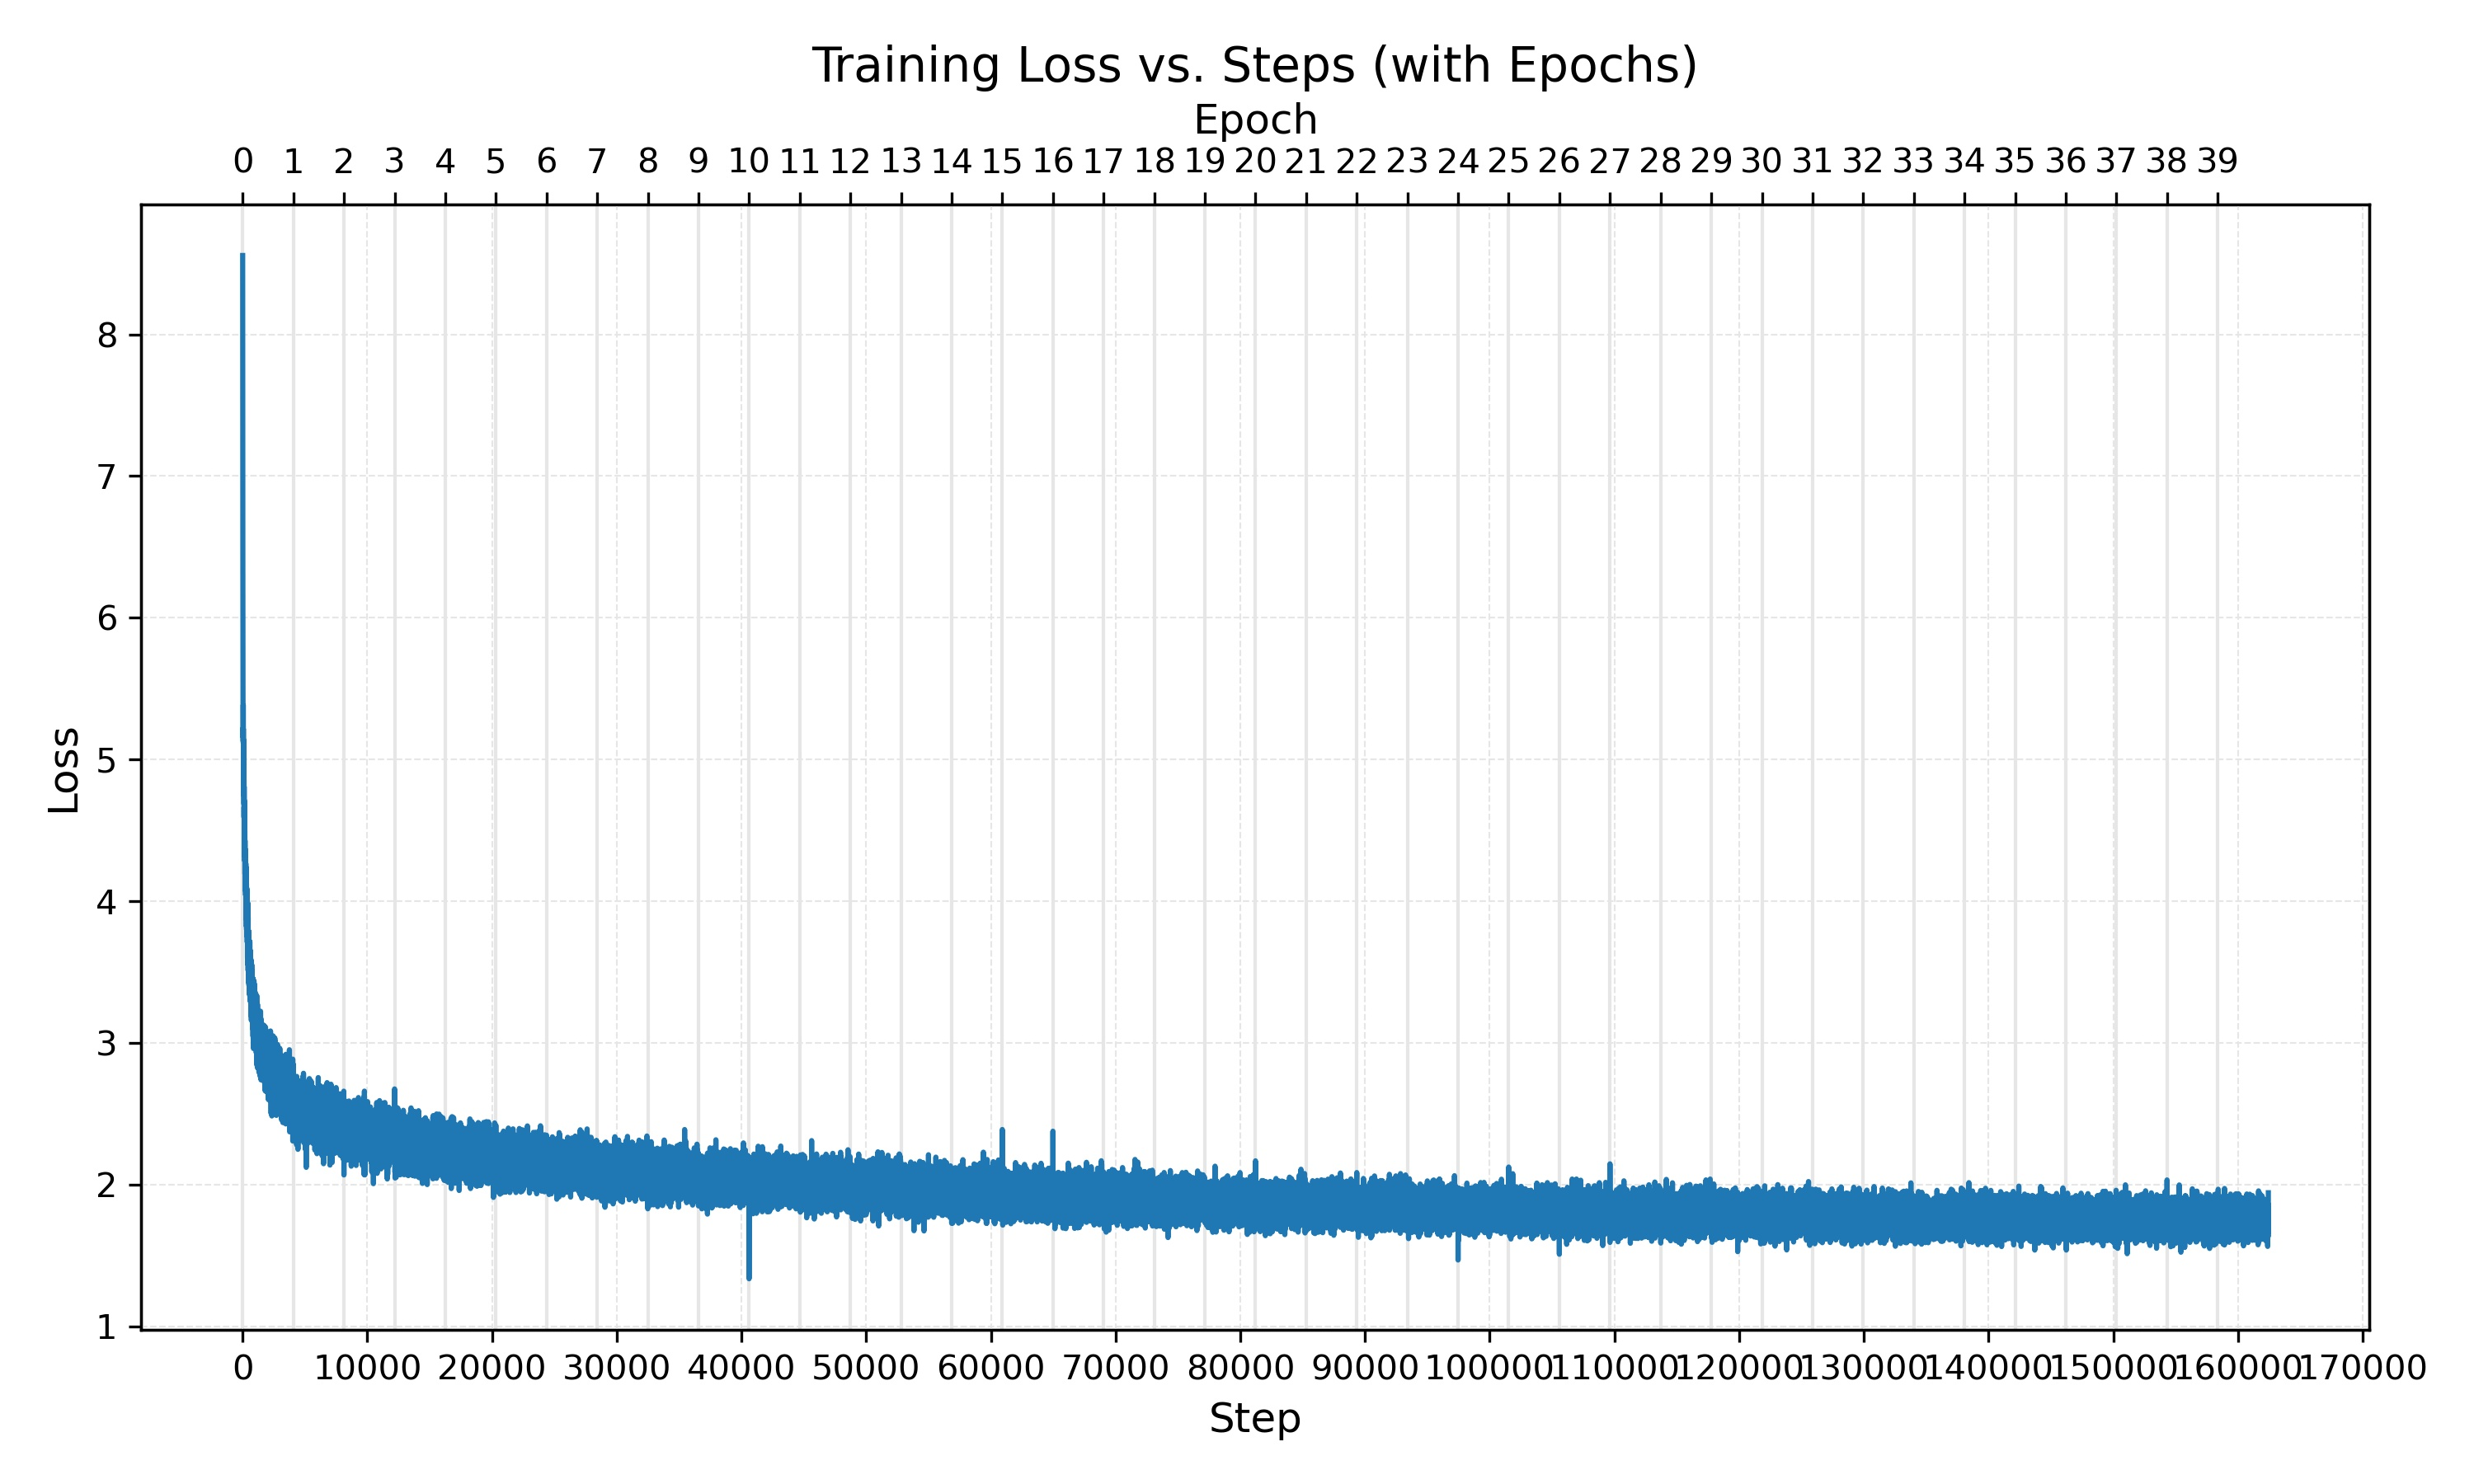
\includegraphics[width=0.8\linewidth]{Figures/model1_loss.jpg}
    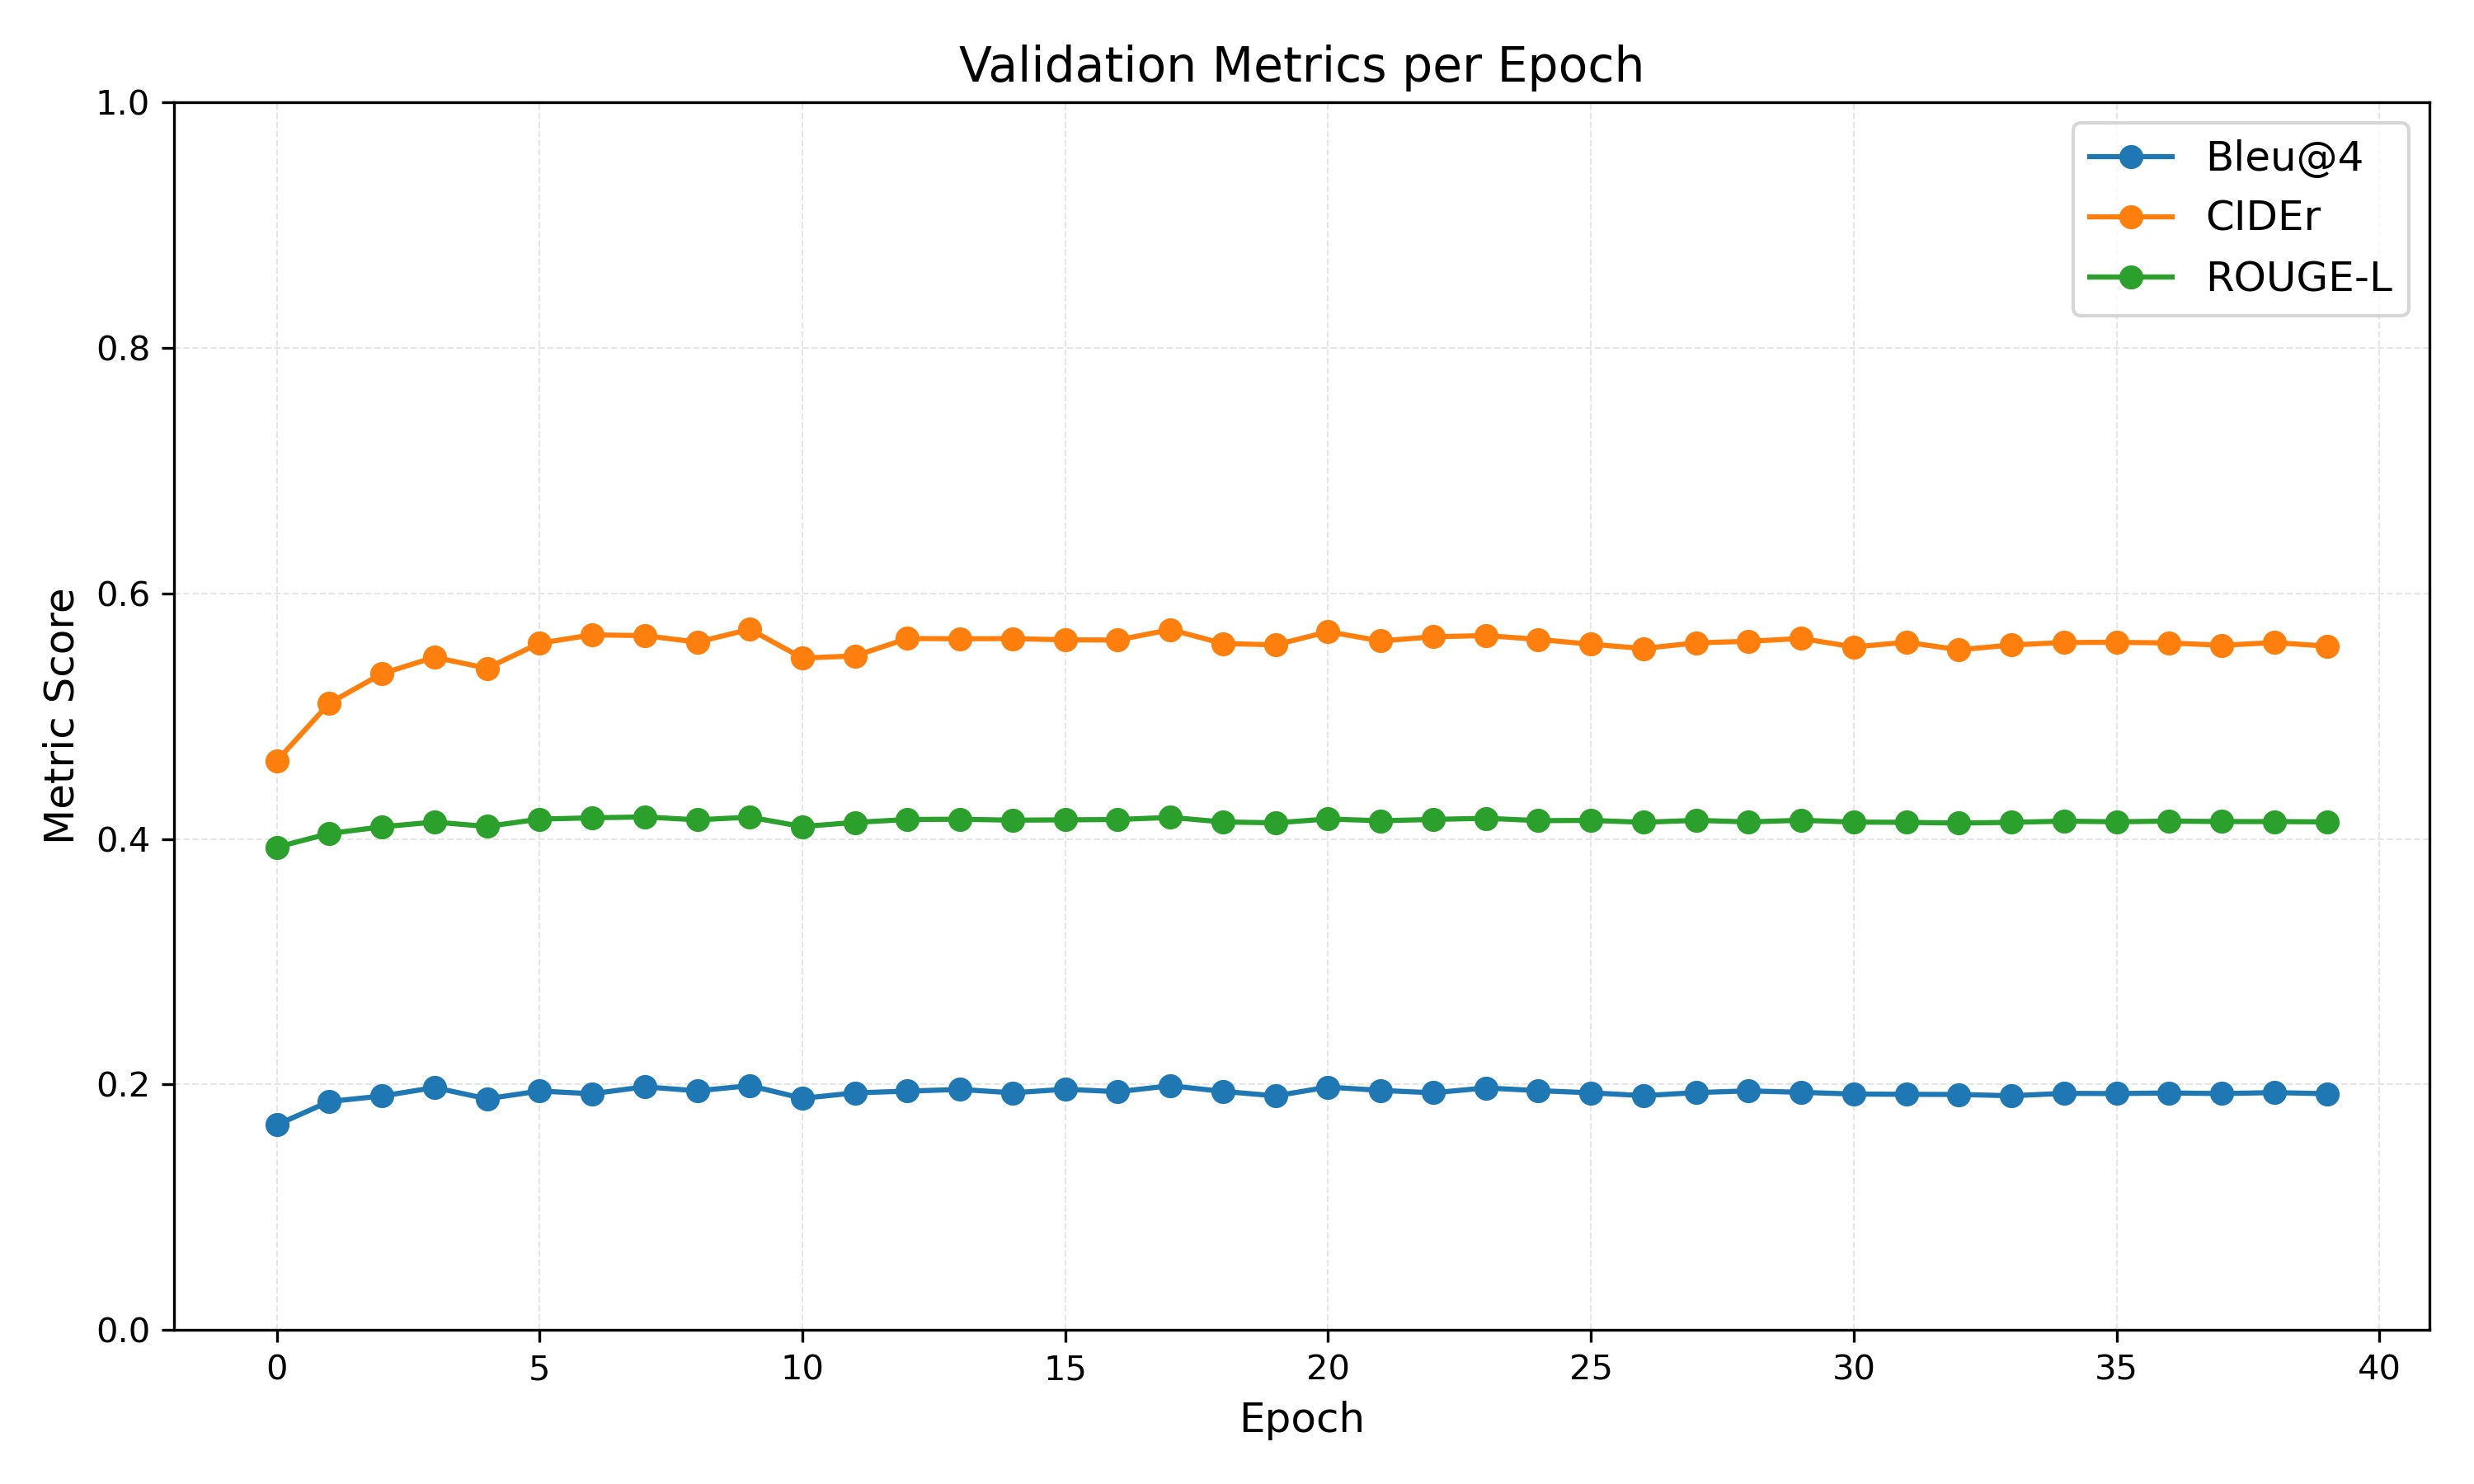
\includegraphics[width=0.8\linewidth]{Figures/model1_metrics.jpg}
    \caption{Per epoch plots for vanilla RNN-model}
    \label{fig:plot_model1}
\end{figure}

\subsection*{Model 2: LSTM model}

The best CIDEr score for the second model was 0.58599, achieved at epoch 5.
The best achieved Bleu@4 score was 0.20110, this time at epoch 10.
Loss and metrics plots per epoch for model 2 is provided in Figure \ref{fig:plot_model2}.
Furthermore, we have provided 5 examples of images with good captions from model 2 (Figure \ref{fig:captioned_images}), and two examples of images where the captions are not as good (Figure \ref{fig:bad_captioned_images}).
In general the captions seem to be relatively good.

\begin{figure}[H]
    \centering
    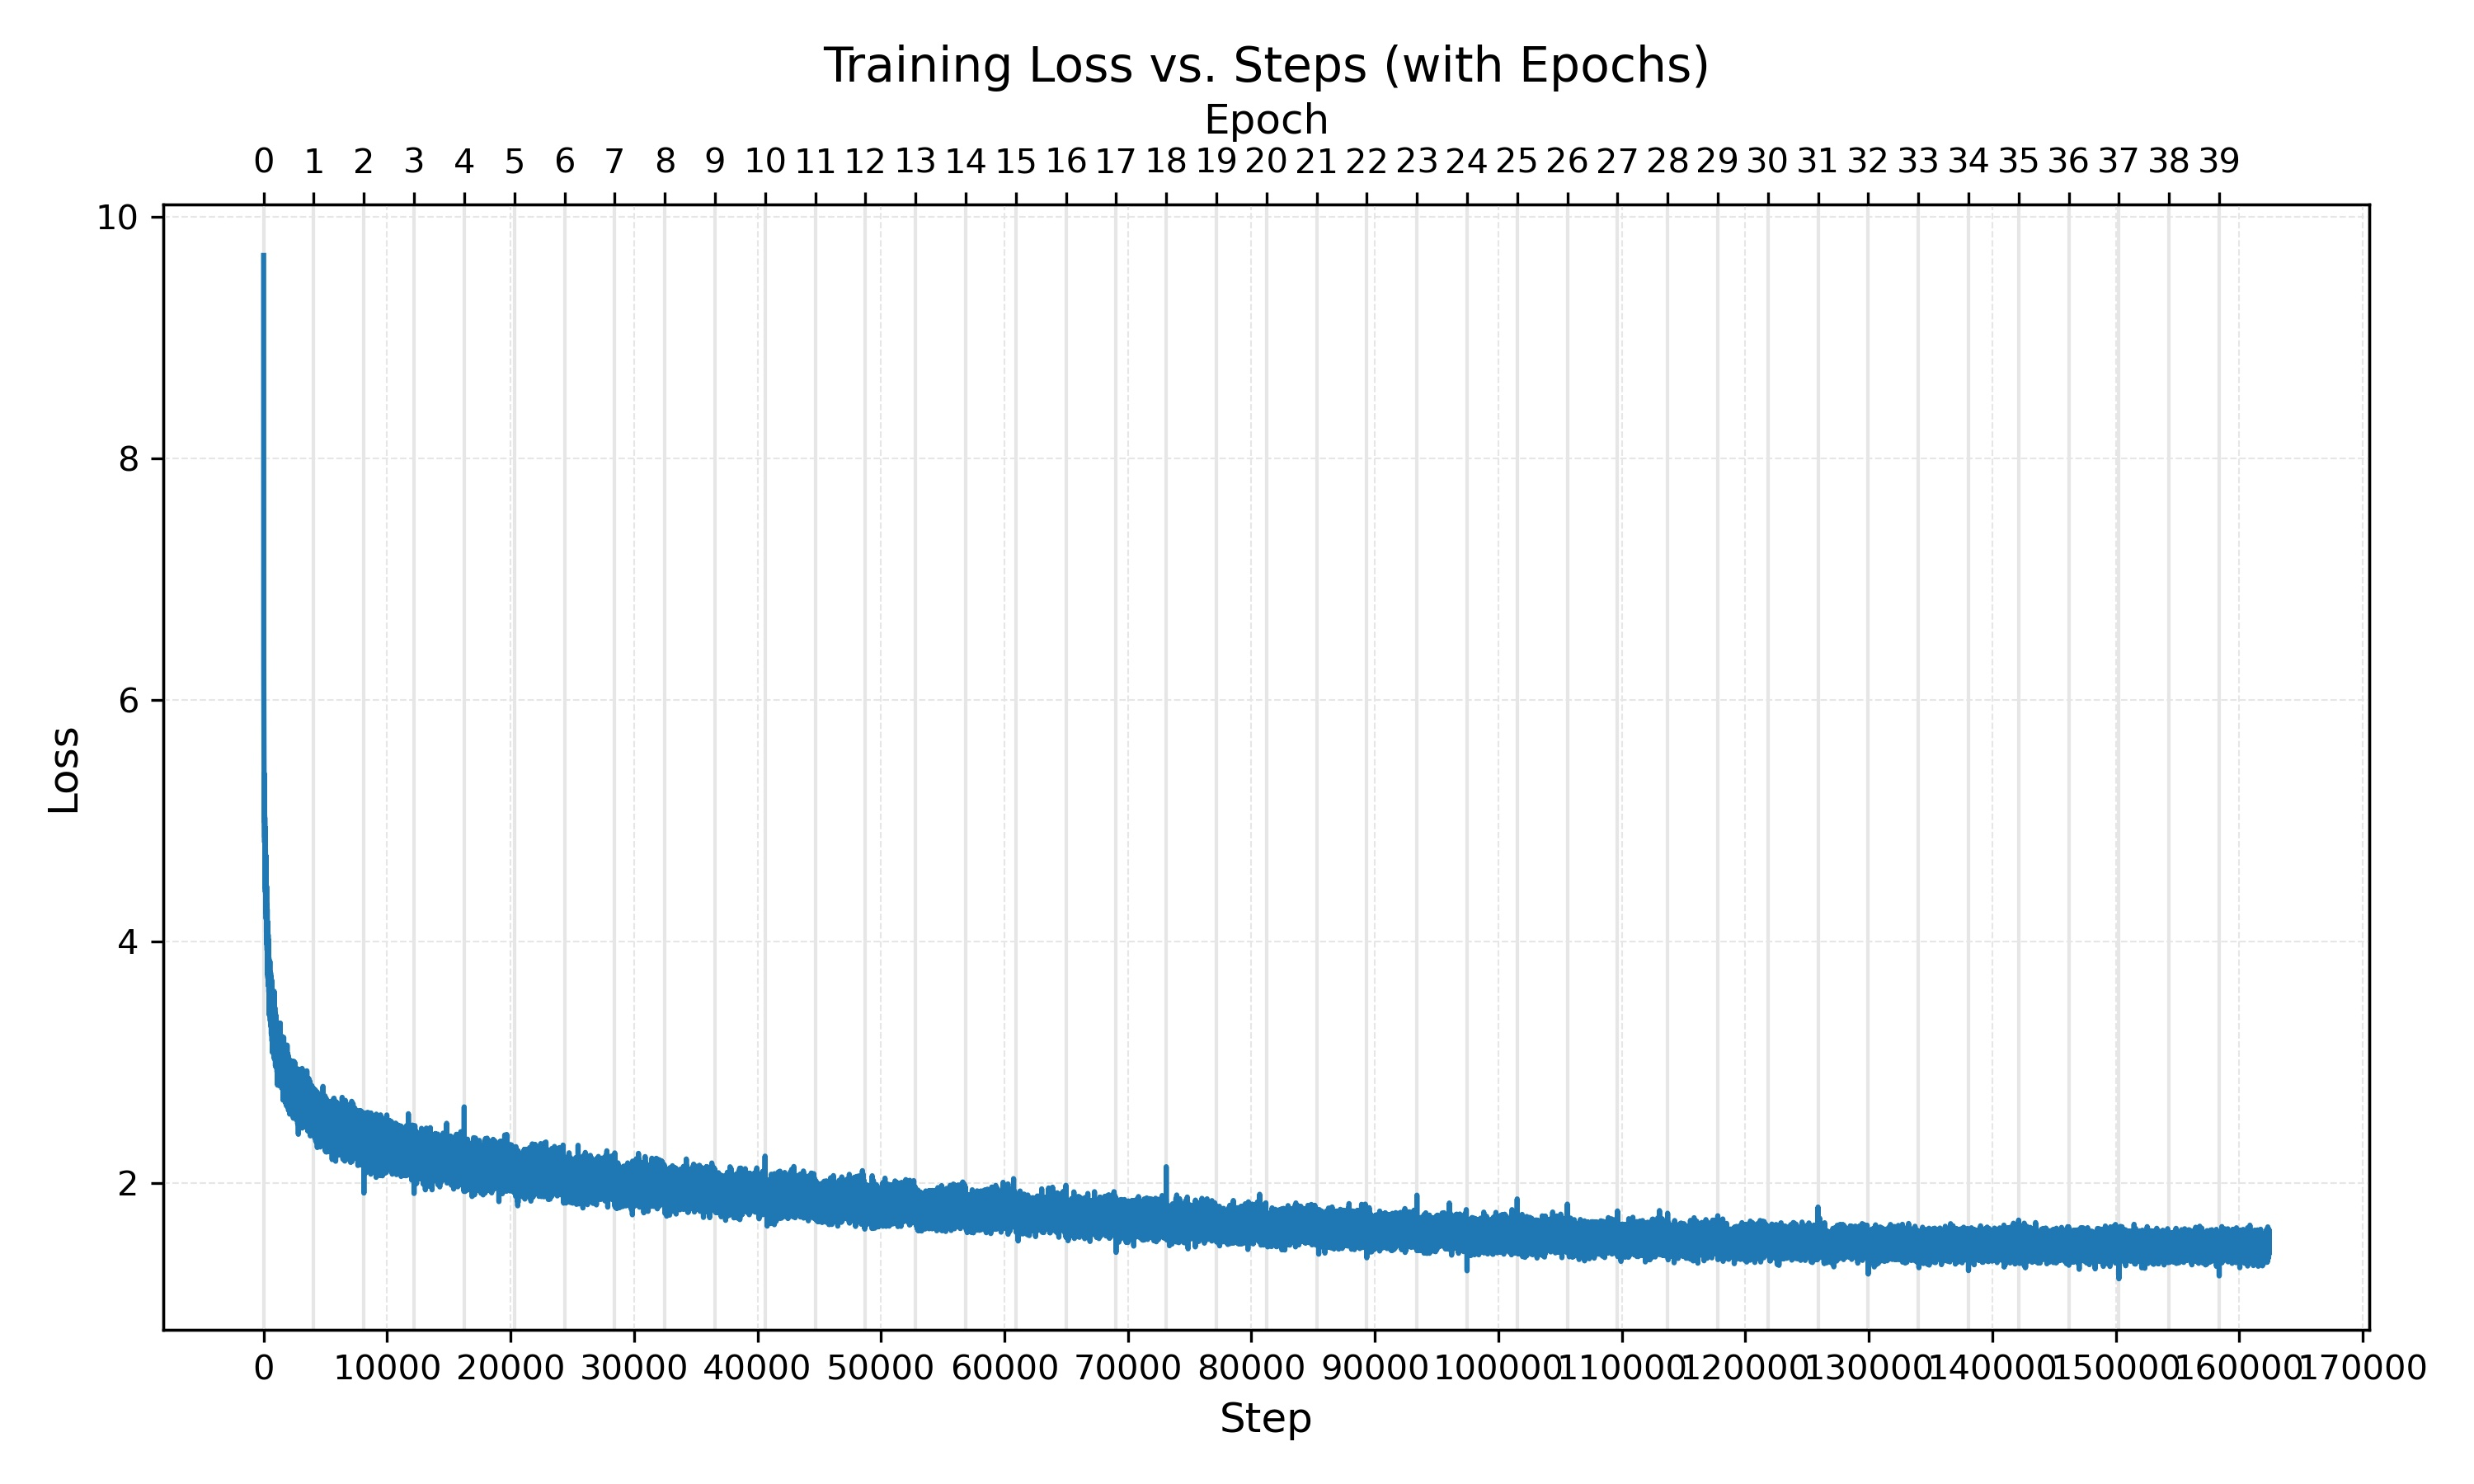
\includegraphics[width=0.8\linewidth]{Figures/model2_loss.jpg}
    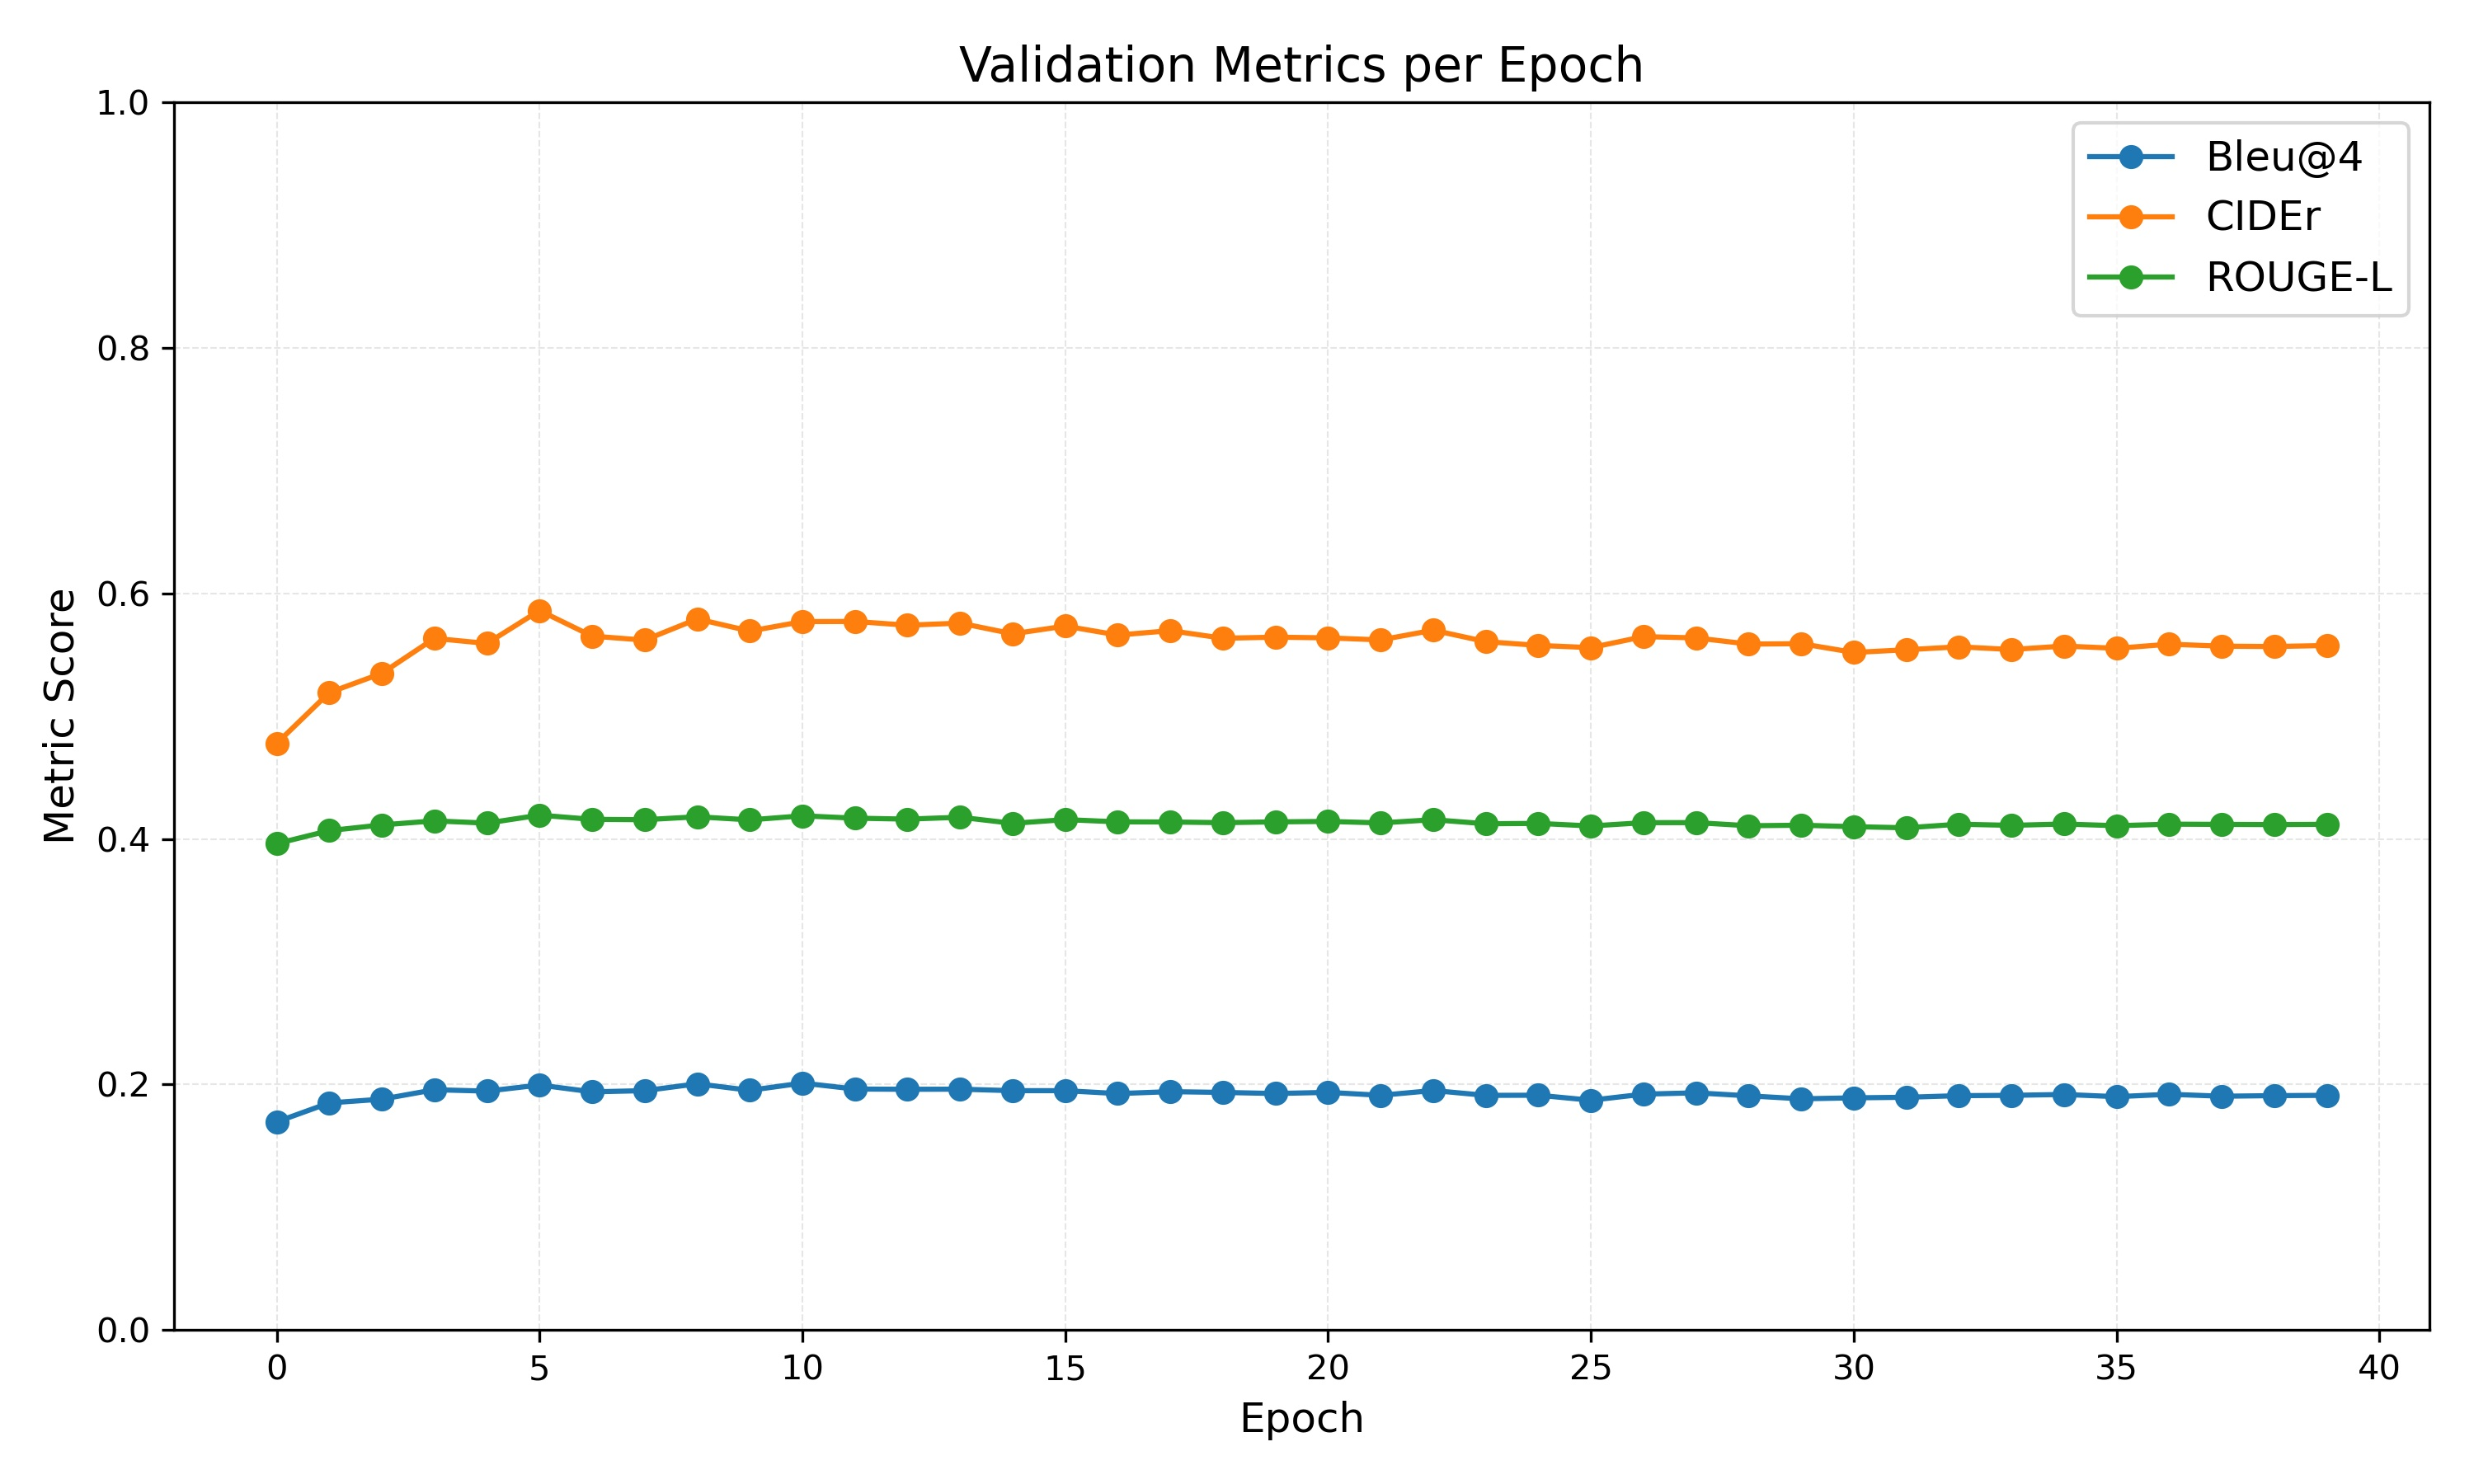
\includegraphics[width=0.8\linewidth]{Figures/model2_metrics.jpg}
    \caption{Per epoch plots for LSTM-model}
    \label{fig:plot_model2}
\end{figure}

\begin{figure}[H]
    \centering
    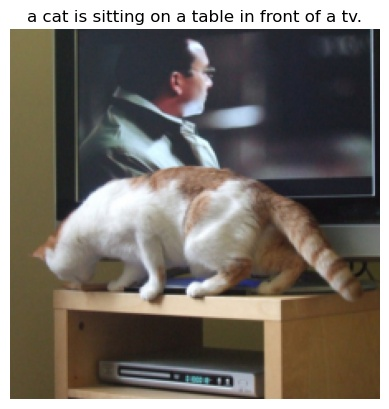
\includegraphics[width=0.45\linewidth]{Images/25560.jpg}
    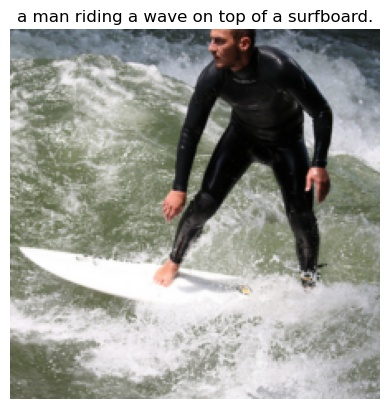
\includegraphics[width=0.45\linewidth]{Images/115898.jpg}
    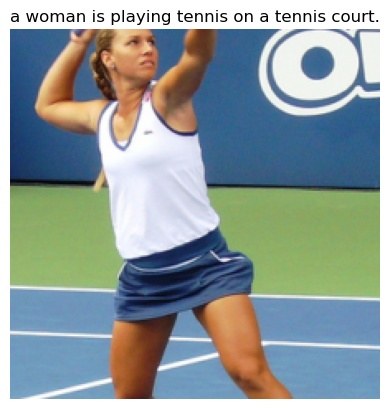
\includegraphics[width=0.45\linewidth]{Images/127270.jpg}
    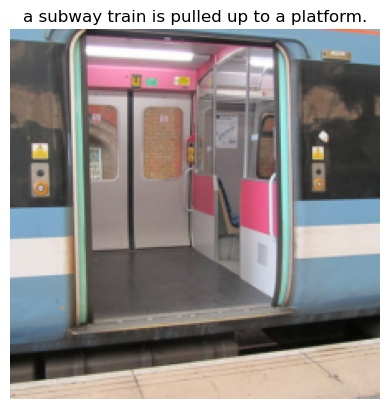
\includegraphics[width=0.45\linewidth]{Images/213816.jpg}
    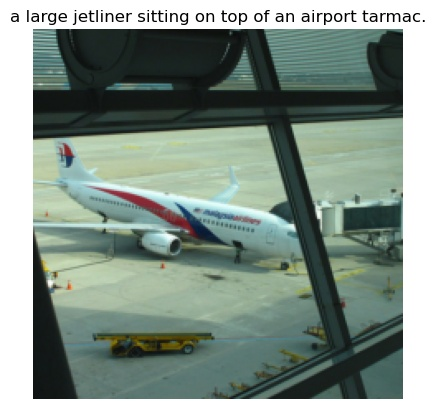
\includegraphics[width=0.45\linewidth]{Images/477441.jpg}
    \caption{Examples of well captioned pictures from model 2}
    \label{fig:captioned_images}
\end{figure}

\begin{figure}[H]
    \centering
    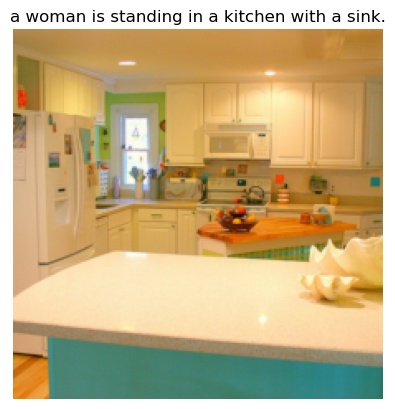
\includegraphics[width=0.45\linewidth]{Images/540502.jpg}
    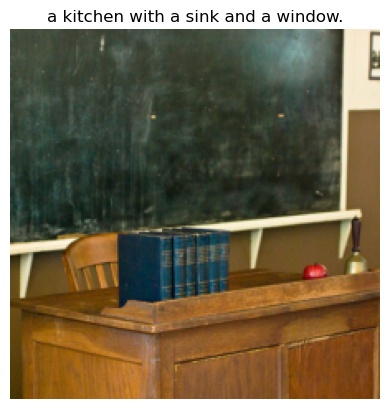
\includegraphics[width=0.45\linewidth]{Images/17182.jpg}
    \caption{Examples of badly captioned pictures from model 2}
    \label{fig:bad_captioned_images}
\end{figure}

\subsection*{Model 3: LSTM with attention}

The third model reached its best CIDEr score at epoch 14, with a value of 0.58654.
The best Bleu@4 score was 0.20748, achieved at epoch 6.
Judging only from the CIDEr and Bleu@4 metrics, model 3 seems to perform best of the three models, which is not surprising as it is the most complex model.

Loss and metrics plots per epoch for model 3 is provided in Figure \ref{fig:plot_model3}.

\begin{figure}[H]
    \centering
    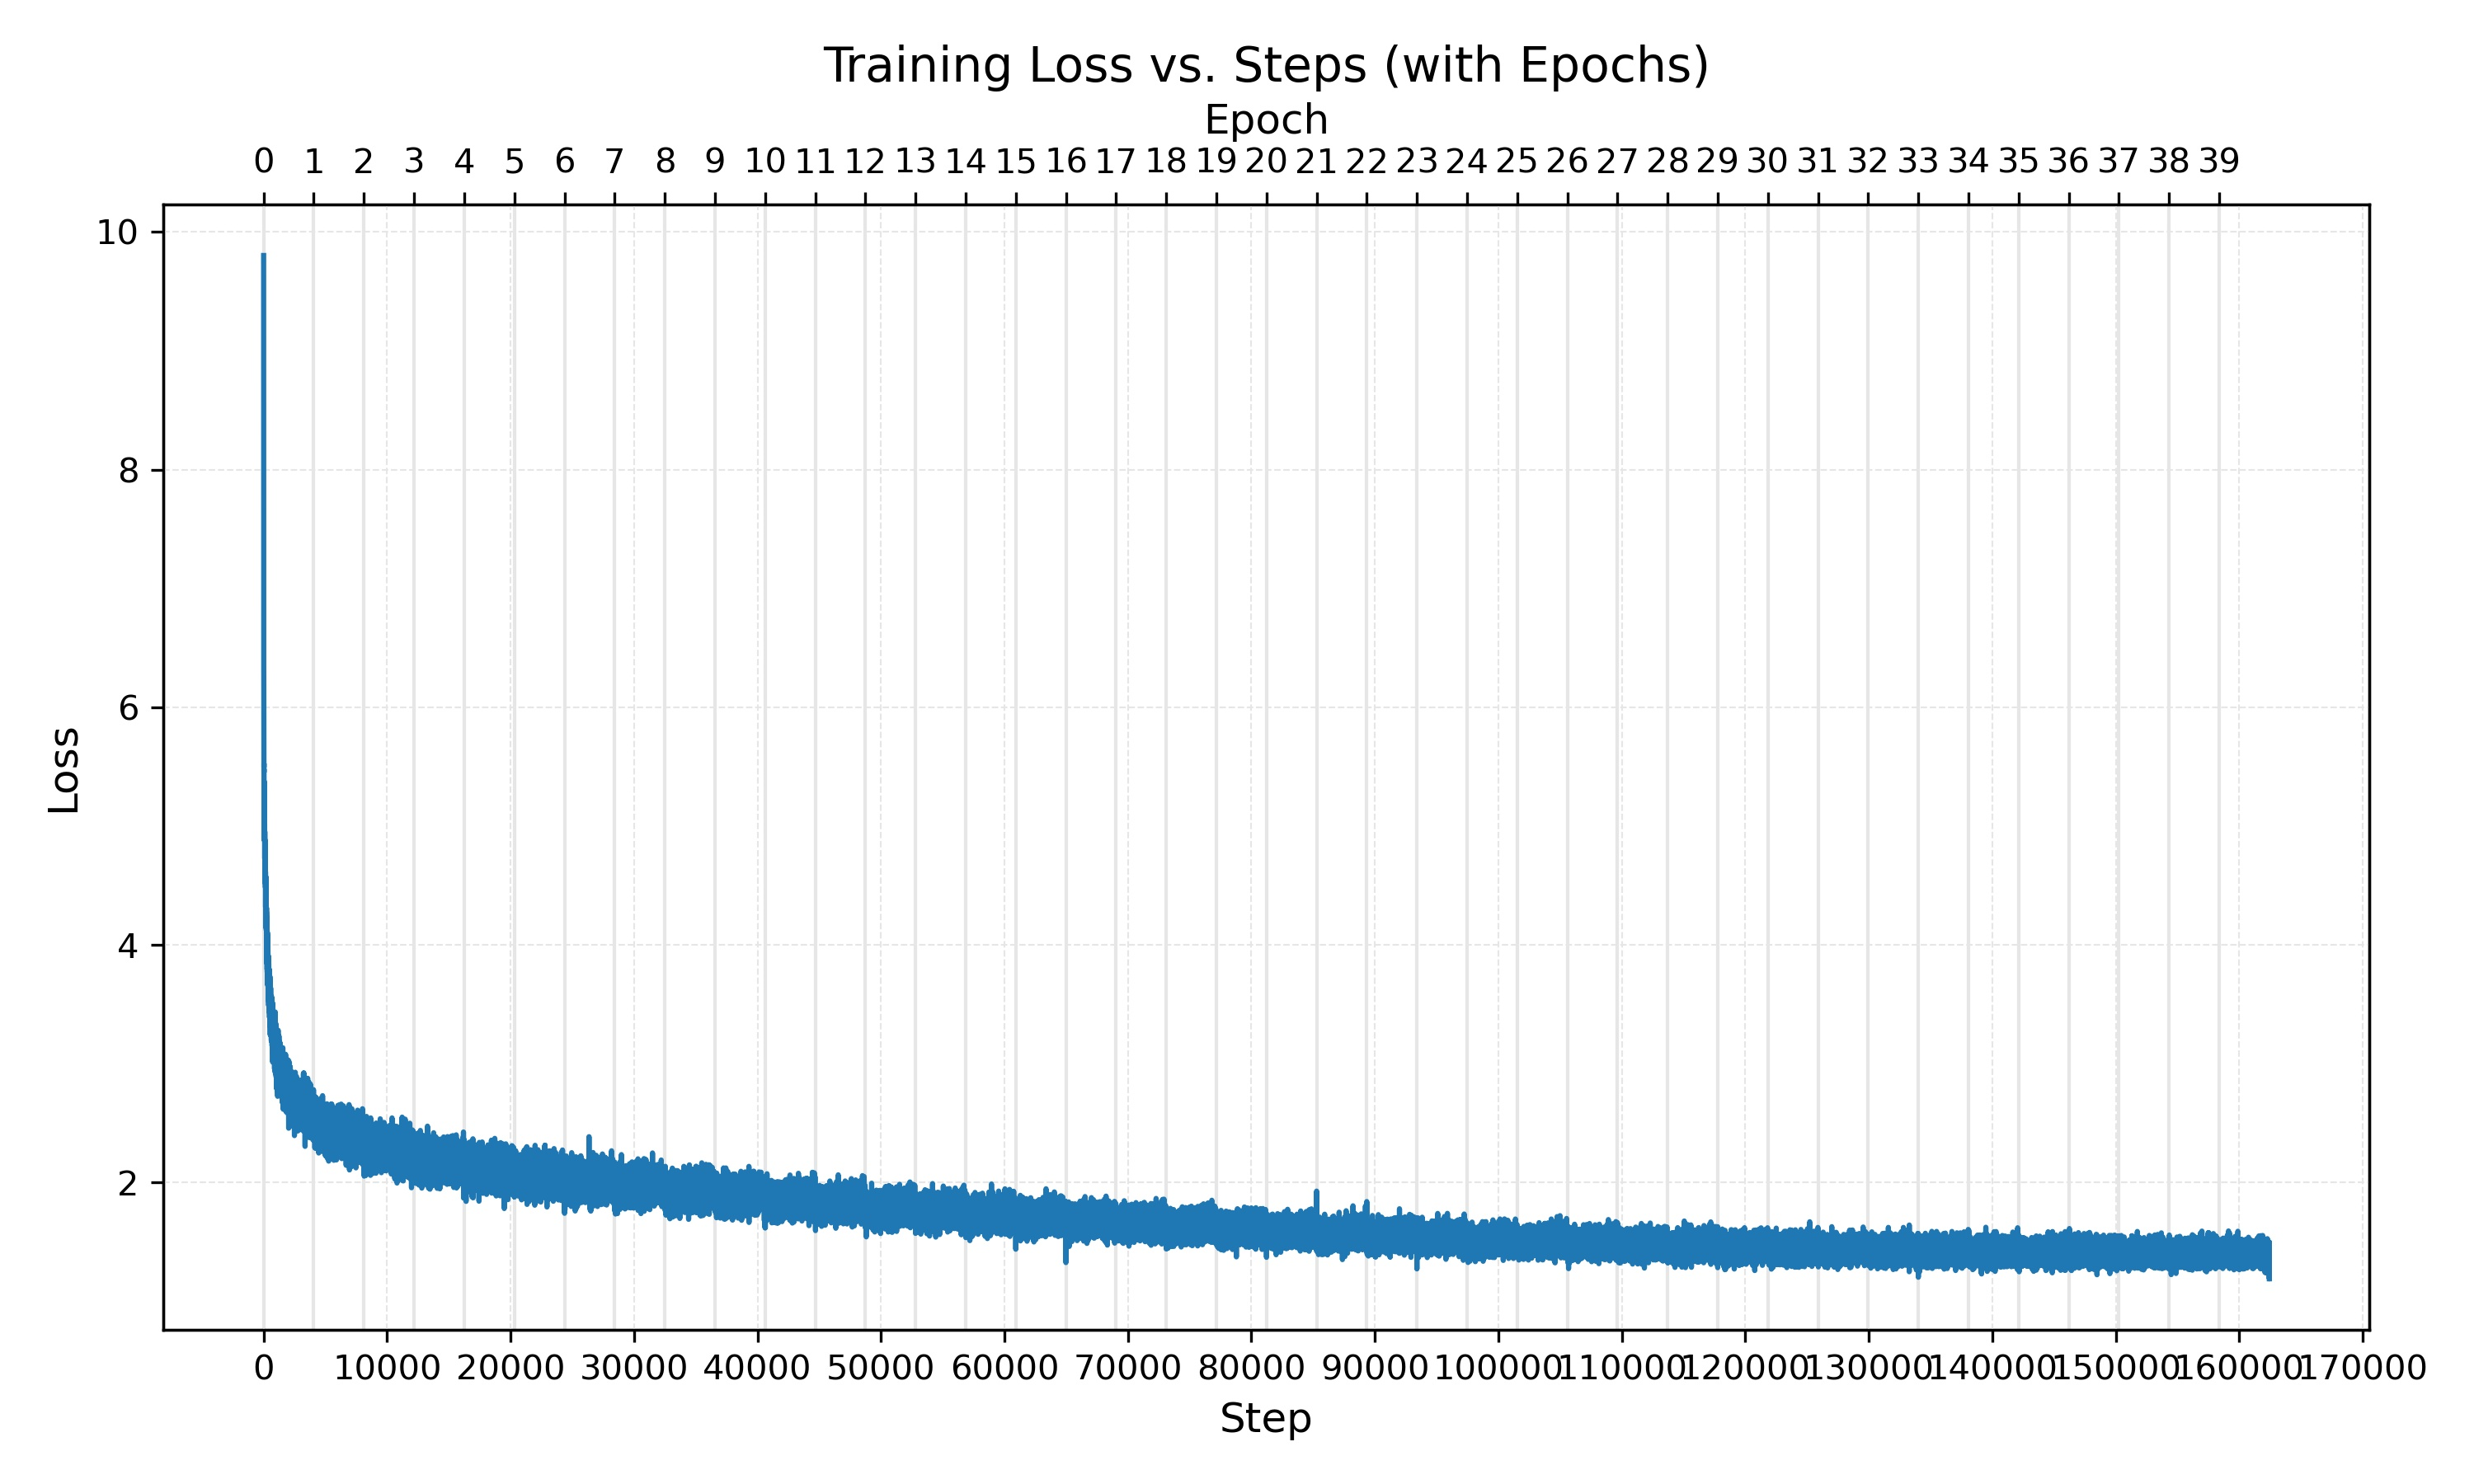
\includegraphics[width=0.8\linewidth]{Figures/model3_loss.jpg}
    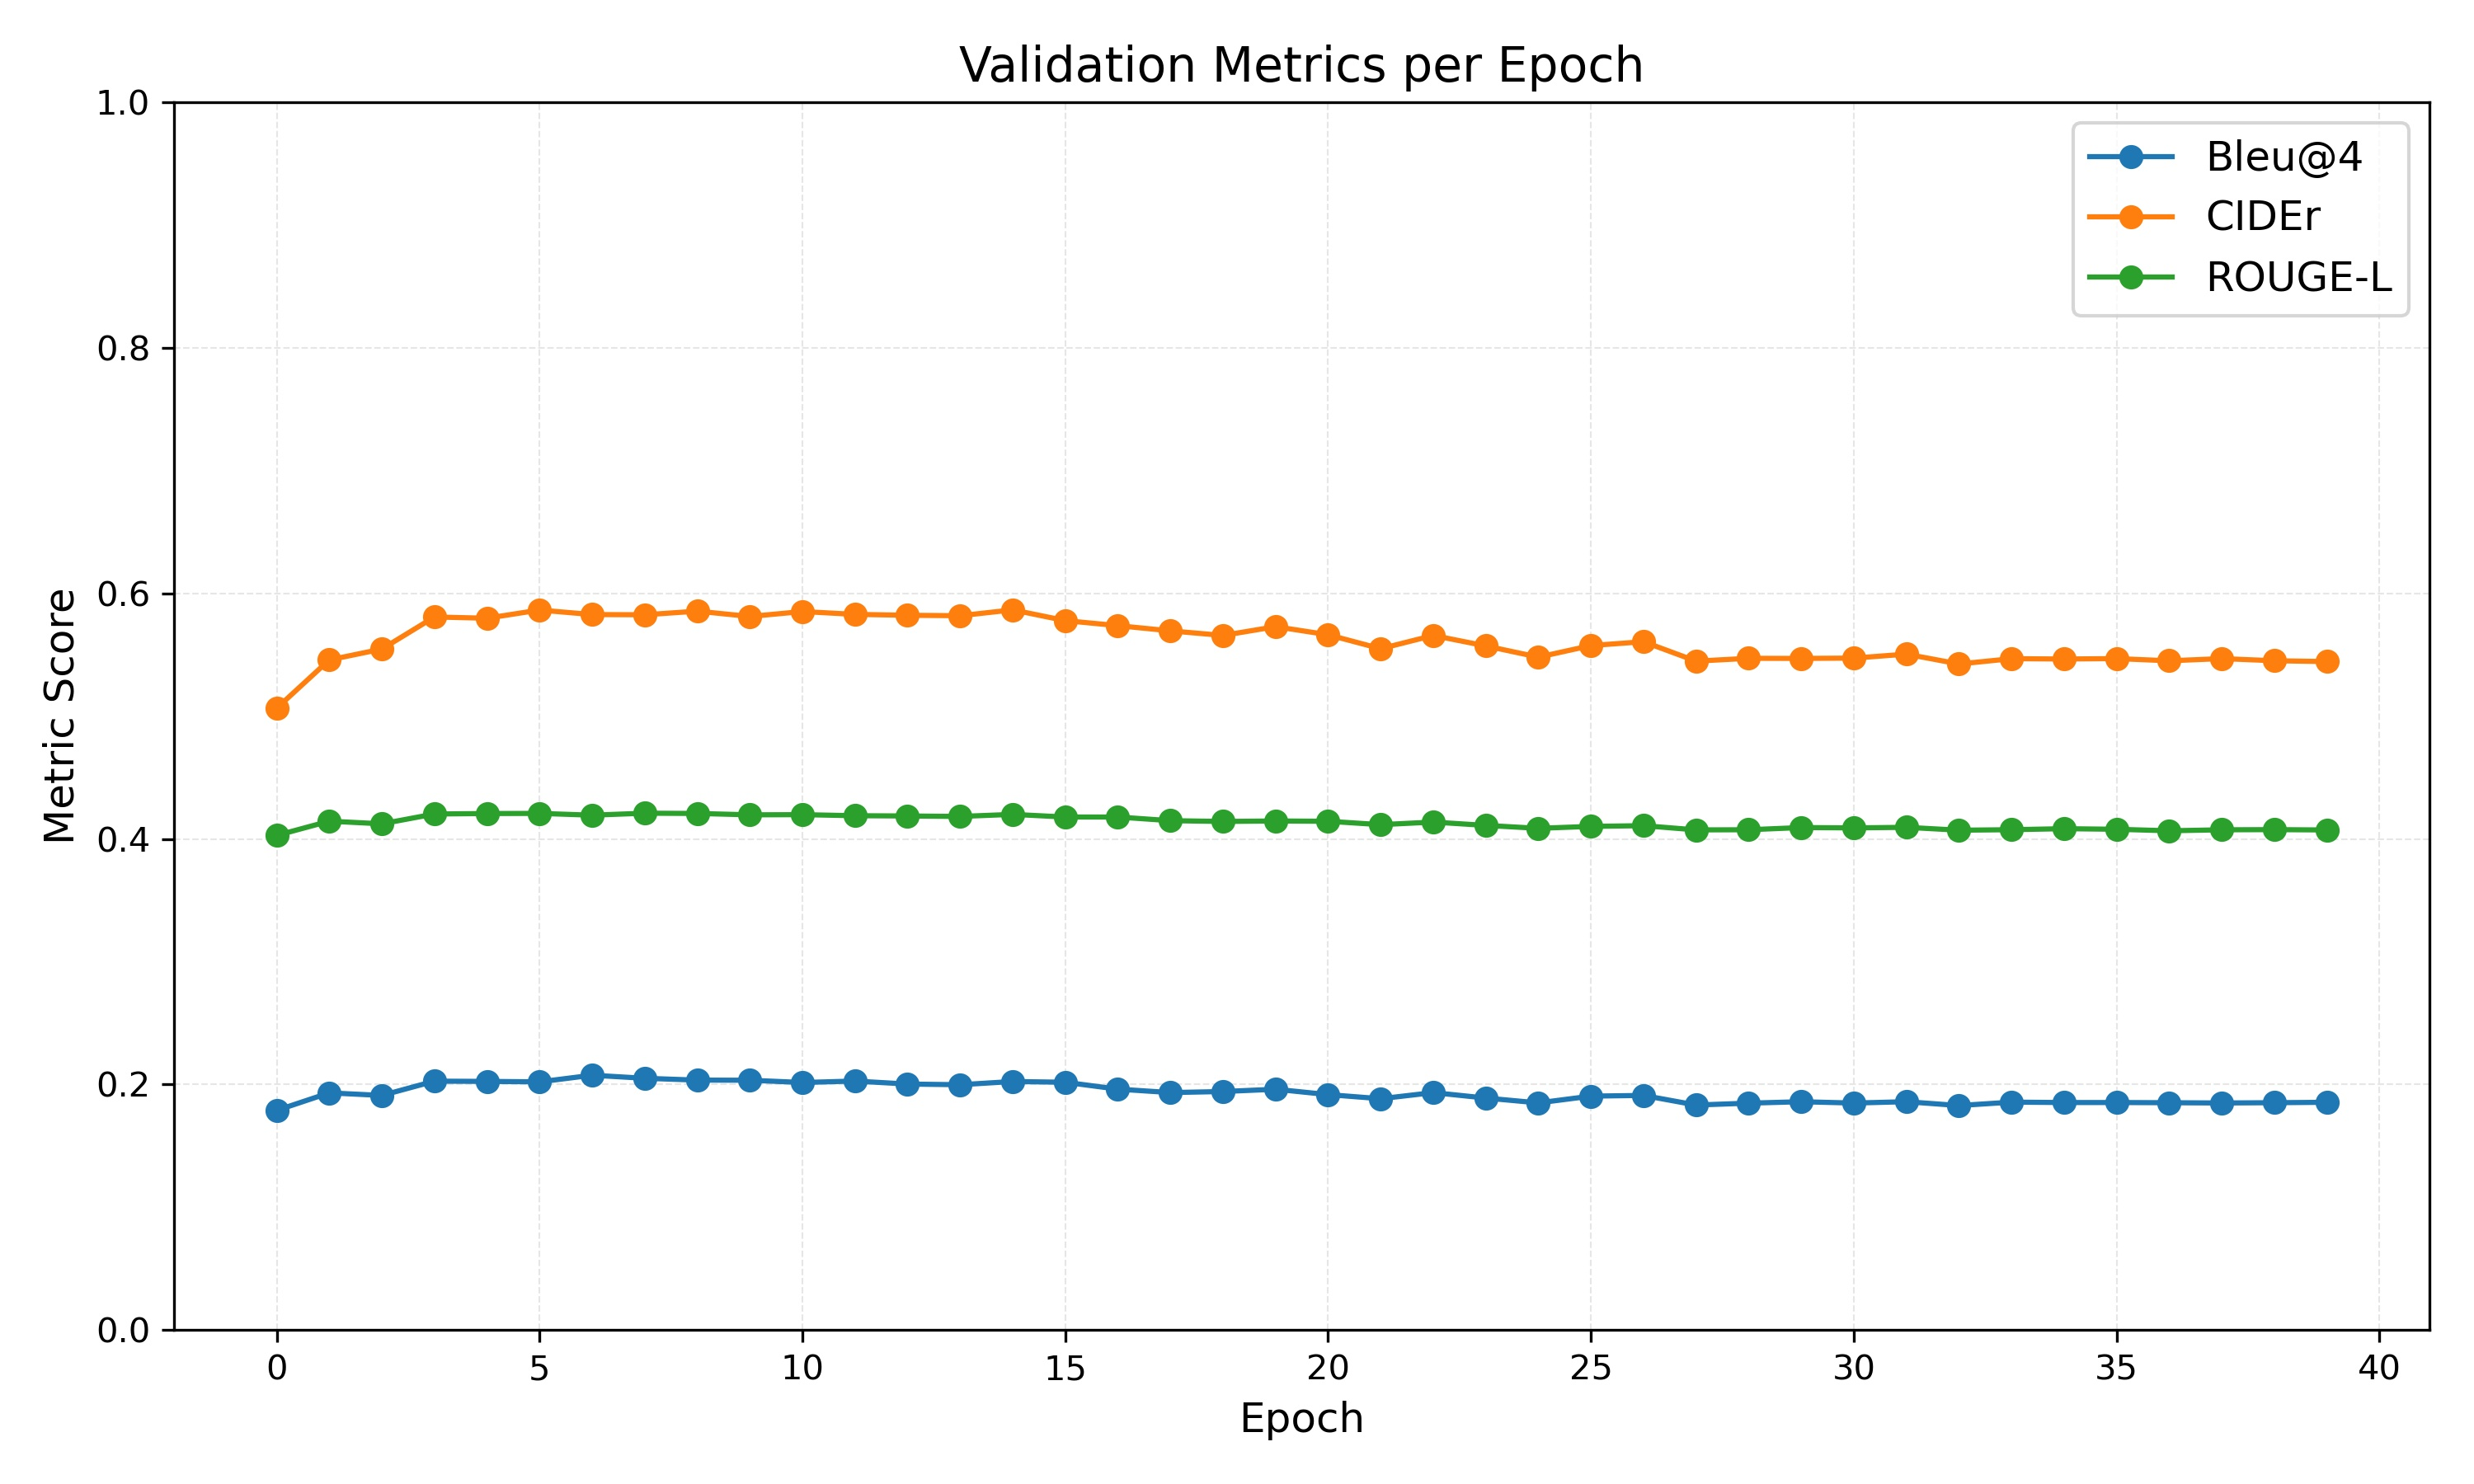
\includegraphics[width=0.8\linewidth]{Figures/model3_metrics.jpg}
    \caption{Per epoch plots for LSTM-model with attention}
    \label{fig:plot_model3}
\end{figure}





\end{document}

